\documentclass[11pt,a4paper]{article}
\usepackage[utf8]{inputenc}
\usepackage{amsmath}
\usepackage{parskip}
\usepackage{amsfonts}
\usepackage{amssymb}
\usepackage{makeidx}
\usepackage{graphicx}
\usepackage{float}
\usepackage{lmodern}
\usepackage{kpfonts}
\usepackage{xcolor}
\usepackage{cancel}
\usepackage{mathtools}
\usepackage{schemata}
\usepackage{cancel}
\providecommand{\abs}[1]{\lvert#1\rvert}%Sirve para colocar valores absolutos
\providecommand{\norm}[1]{\lVert#1\rVert}%Sirve para colocar módulo
\usepackage[left=2.00cm, right=2.00cm, top=2.00cm,bottom=2.00cm]{geometry}
\author{Harold Alessander Jhon Zambrano Quispe}
\title{SOLUCIONARIO DE LA TAREA 1}
\begin{document}
   \begin{titlepage}%Habilita una pagina sin enumerar.
	\begin{center}
	 {\huge \textbf{Universidad Nacional de Ingeniería}}\\
	 \vspace{3mm}
	  {\Large {Facultad de Ingeniería Eléctrica y Electrónica}}\\
	\vspace{-5mm}	 
	 \begin{figure}[h]
	 	\centering 
	 	
\includegraphics[scale=0.5]{Logo UNI}
	 \end{figure}
	 \vspace{-6mm}
	{\Large {Especialidad de Ingeniería de Telecomunicaciones}}\\
	\vspace{3mm}
	{\Large \textbf{"Laboratorio 1 de Análisis de Señales y Sistemas"}}\\
	\vspace{8mm}
	\begin{flushleft}
	{\Large {\textbf{Curso}: Análisis de Señales y Sistemas}}\\
	\vspace{8mm}		
	{\Large {\textbf{Código del Curso}: EE410-M}}\\	
	\vspace{8mm}	
	{\Large {\textbf{Docente}: Manuel Arevalo Villanueva}}\\
	\vspace{8mm}	
	{\Large {\textbf{Integrantes}: 
	Gian Carlos Chancavilcas Osores - 20191108K\\
	\vspace{4mm}
	\hspace{3cm}Julio Cesar Luna Yabarrena - 20130346I\\ 
	\vspace{4mm}
	\hspace{3cm}Harold Alessander Jhon Zambrano Quispe - 20191351B}}\\
	\vspace{8mm}	
	\end{flushleft}
	\vspace{10mm}
	{\Huge {\textbf{2021-I}}}\\
	\end{center}
\end{titlepage}
%Se debe compilar desde la funcion principal
   \begin{titlepage}%Habilita una pagina sin enumerar.
	\begin{center}
	 {\huge \textbf{INDICE}}\\
   \begin{flushleft}
   \vspace{8mm}
	{\Large {\textbf{1. MARCO TEÓRICO}}}\\
	\vspace{8mm}		
	{\Large {\textbf{2. PROBLEMAS}}}\\	
	\vspace{8mm}	
	{\Large {\textbf{3. CONCLUSIONES}}}\\
	\vspace{8mm}
	{\Large {\textbf{4. BIBLIOGRAFIA}}}
	\vspace{8mm}	
	\end{flushleft}
	\end{center}
\end{titlepage}
   \section{{MARCO TEÓRICO}}{
	\large{
	\begin{enumerate}
	\item[\textbf{a.}]
	\begin{flushleft}
\textbf{CONVOLUCIÓN DISCRETA}
\end{flushleft}
Convolución es un valor que se extiende a todos los sistemas que son invariantes linear del tiempo (LTI - Linear Time Invariant). La idea de convolución discreta es la misma que la de convolución continua. Por esta razón, puede ser de gran ayuda el ver las dos versiones para que usted entienda la extrema importancia del concepto. Recuerde que la convolución es un instrumento poderoso al determinar el resultado de un sistema después de saber la una entrada arbitraria y la respuesta al impulso del sistema. 
\begin{flushleft}
\textbf{SUMA DE CONVOLUCIÓN}
\end{flushleft}
Como ya ha sido mencionado, la suma de convolución provee una manera matemáticamante concisa para expresar el resultado de un sistema LTI, basado en una entrada arbitraria para una señal discreta y también el saber la respuesta del sistema. La suma de convolución es expresada como:
$$\boxed{y[n]=x[n]*h[n]=\sum_{k=-\infty}^{\infty}x[k]h[n-k]}$$

	\item[\textbf{b.}]
	\textbf{TRANSFORMADA Z}\\\\
	Para aplicar la transformada Z se debe utilizar la definición.

\begin{center}
$\boxed{\mathcal{Z}\{f[n]\}=\sum_{n=-\infty}^{\infty}\frac{f[n]}{Z^n}}$
\end{center}

Con la siguiente definición se podrá obtener algunos resultados notables

\begin{itemize}

    \item $\mathcal{Z}\{\delta[n]\}=\sum_{n=-\infty}^{\infty}\frac{\delta[1]}{Z^n}=1$\\
    \item $\mathcal{Z}\{r^nu[n]\}=\sum_{n=-\infty}^{\infty}\frac{r^nu[n]}{Z^n}=\sum_{n=0}^{\infty}\frac{r^n}{Z^n}=\frac{z}{z-r}$\\
    Donde $|r|\leq1$ además $r\in\mathrm{C}$\\
    \item $\mathcal{Z}\{r^nnu[n]\}=\sum_{n=-\infty}^{\infty}\frac{r^nnu[n]}{Z^n}=\sum_{n=0}^{\infty}\frac{r^nn}{Z^n}=\frac{z}{(z-r)^2}$\\
    Donde $|r|\leq1$ además $r\in\mathbf{C}$\\
    
\end{itemize}

De igual manera se puede demostrar algunas propiedades como

\begin{itemize}

    \item $\mathcal{Z}\{C_1f_1[n]+C_2f_2[n]\}=C_1\mathcal{Z}\{f_1[n]\}+C_2\mathcal{Z}\{f_2[n]\}=C_1F_1(z)+C_2F_2(z)$\\
    \item $\mathcal{Z}\{f[n-k]\}=\frac{\mathcal{Z}\{f[n]\}}{z^k}=\frac{F(z)}{z^n}$
  
\end{itemize}
	
	\newpage
	\item[\textbf{c.}]
	\textbf{TRANSFORMADA DE LAPLACE}\\\\
	\textbf{DEFINICIÓN DE LA TRANSFORMADA DE LAPLACE}\\\\
	Sea $F(t)$ una función de t definida para $t>0$. La transformada de Laplace de $F(t)$, denotado por $\mathcal{L}{F(t)}$, se define como:
	\begin{center}
	\boxed{\mathcal{L}{\lbrace F(t)\rbrace}=f(s)=\int_{0}^{\infty} e^{-st} F(t)dt}
	\end{center}
	En general, $f(s)$ existe cuando $s > \alpha$ donde $\alpha$ es cierta constante.\\
	Donde: $\mathcal{L}$ se llama el \textbf{operador de la transformada de Laplace}\\
	
	\textbf{DEFINICIÓN DE LA TRANSFORMADA INVERSA DE LAPLACE}\\\\
	Si la transformada de Laplace de una función $F(t)$, es $f(s)$. es decir $\mathcal{L}{F(t)}=f(s)$,entonces $F(t)$ se llama una \textbf{transformada inversa de Laplace} de (s) y se expresa por:
	\begin{center}
	\boxed{F(t)=\mathcal{L^{-}}{\lbrace f(s) \rbrace}}
	\end{center}
	Donde: $\mathcal{L^{-}}$ se llama el \textbf{operador de la transformada inversa de Laplace}
	\end{enumerate}
	}}
\newpage
	\section{PROBLEMAS}{
	\large{
	\begin{enumerate}
	%Problema 1
	\item[\textbf{1.}]
\textbf{Sea $f(t)=u(t)-u(t-3)$ la señal pulso rectangular , $g(t)= e^{-2t}u(t) , 0\leq t\leq 5$ la  amortiguacion exponencial y sea $h(t)$ la señal  pulso triangular definida asi :}

\[h(t)=\left\{ \begin{array}{lccc}
             0 &   si  & t \leq 0 \\
             \\ t &  si & 0 < t < 1 \\
             \\ 2-t &  si  & 1 < t < 2\\
             \\  0 & si &  t < 2
             \end{array}
   \right.
\]
\textbf{Usando el MATLAB grafique las señales  en tiempo continuo $f(t) , g(t) , h(t)$\newline
Encuentre en terminos de  de t y de la señal escalon  unitario  las siguientes convoluciones: $f(t)*g(t) ,f(t)*h(t) ,g(t)*h(t)\newline  $
Usando el matlab y el comando \textit{conv} grafique las convoluciones $f(t)*f(t),\ f(t)*g(t), \ g(t)*g(t),\ g(t)*h(t),\ h(t)*h(t)$.}\newline

\textbf{Solución:}\\\\
\textbf{función f(t)=u(t)-u(t-3)=rectpuls(t-1.5)}
\begin{figure}[h]
    \centering
    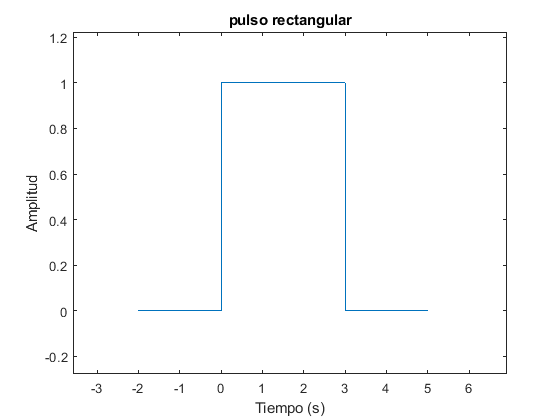
\includegraphics[scale=0.80]{fig1.png}
    \caption{grafica de la funcion f(t)}
    \label{fig:my_label}
\end{figure}

\newpage


\textbf{funcion $g(t)=e^{-2t}u(t)$}
\begin{figure}[h]
    \centering
    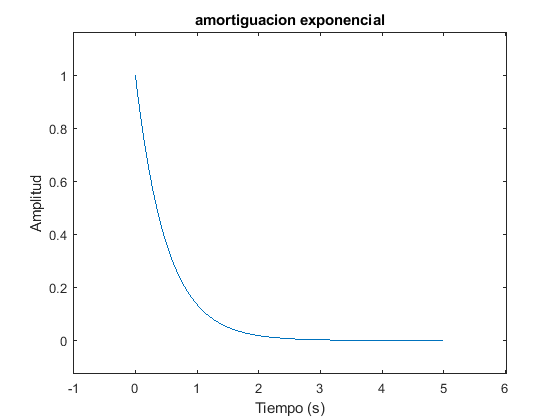
\includegraphics[scale=0.80]{fig2.png}
    \caption{grafica de la funcion g(t)}
    \
\end{figure}



\textbf{funcion $h(t)= \ tripuls(t-1) \ = u_1(t)-2u_1(t-1)+u_1(t-2) $}
\begin{figure}[H]
    \centering
    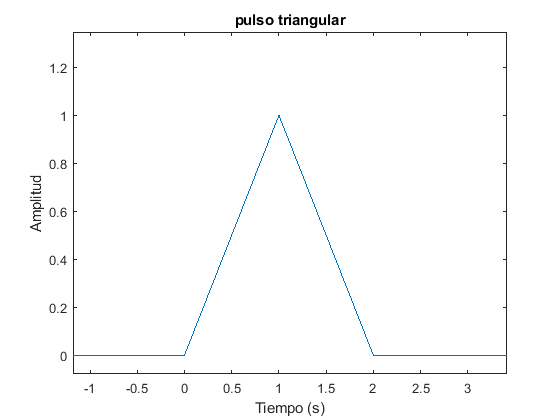
\includegraphics[scale=0.80]{fig3.png}
    \caption{grafica de la funcion g(t)}
\end{figure}
\newpage



Ahora hallaremos las convoluciones de \ $f(t)*g(t) ,f(t)*h(t) ,g(t)*h(t)$\newline \newline
\empty{\underline{\textbf{$f(t)*g(t)$= $\int_{-\infty}^{\infty} g(\tau)f(t-\tau) d\tau  $}}}
\newline$\\
Para  \ t<0$
\begin{figure}[H]
    \centering
    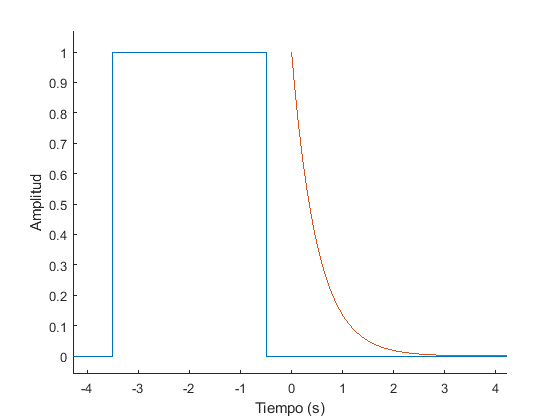
\includegraphics[scale=0.7]{fig4.png}
    \caption{para valores de $ t\ < 0$}
    \label{fig:my_label}
\end{figure}

Vemos que las graficas no se interceptan , por lo tanto $\int_{-\infty}^{\infty} g(\tau)f(t-\tau) d\tau = 0 $\newline


Para   $0 < t < 3$ \\
\begin{figure}[H]
    \centering
    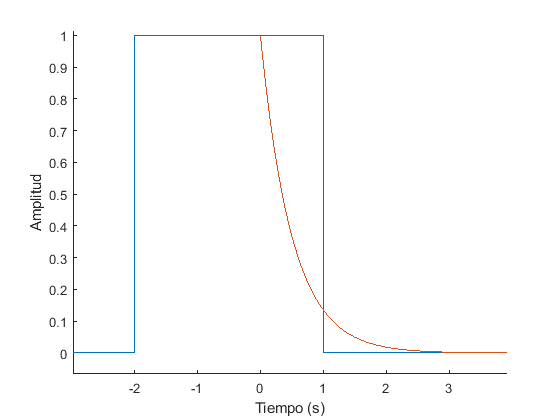
\includegraphics[scale=0.6]{fig5.png}
    \caption{grafica en $0 < t < 3$ }
\end{figure}
$\int_{-\infty}^{\infty} g(\tau)f(t-\tau) d\tau = \int_{0}^{t} e^{-2t}.1 d\tau = \dfrac{1}{2}-\dfrac{e^{-2t}}{2}  $\\
\newpage


Para   $3 < t < 5$ \\
\begin{figure}[H]
    \centering
    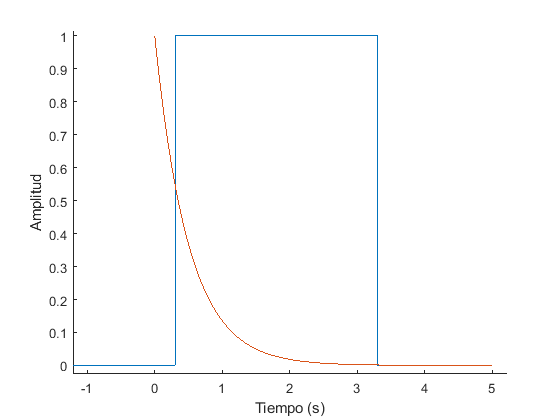
\includegraphics[scale=0.6]{fig6.png}
    \caption{grafica en $3 < t < 5$ }
\end{figure}
$\int_{-\infty}^{\infty} g(\tau)f(t-\tau) d\tau = \int_{-3+t}^{t} \ e^{-2t}.1 d\tau = \ \dfrac{e^{-2t+6}}{2}-\dfrac{e^{-2t}}{2}  $\\
\newline
\newline


Para   $5 < t < 8$ \\
\begin{figure}[H]
    \centering
    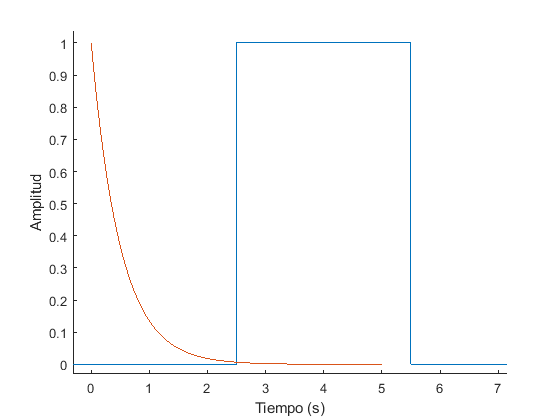
\includegraphics[scale=0.6]{fig7.png}
    \caption{grafica en $5 < t < 8$ }
\end{figure}
$\int_{-\infty}^{\infty} g(\tau)f(t-\tau) d\tau = \int_{-3+t}^{5} \ e^{-2t}.1 d\tau = \ \dfrac{e^{-2t+6}}{2}-\dfrac{e^{-10}}{2}  $\\
\newpage



Para   $8 < t$ \\
\begin{figure}[H]
    \centering
    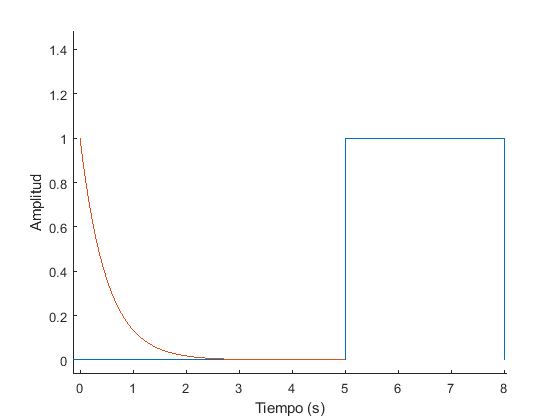
\includegraphics[scale=0.6]{fig8.png}
    \caption{grafica en $5 < t < 8$ }
\end{figure}

$\int_{-\infty}^{\infty} g(\tau)f(t-\tau) d\tau = \int_{8}^{\infty} \ e^{-2t}.1 d\tau = 0  $\\ \newline
la grafica de $f(t)*g(t)$ es

\begin{figure}[H]
    \centering
    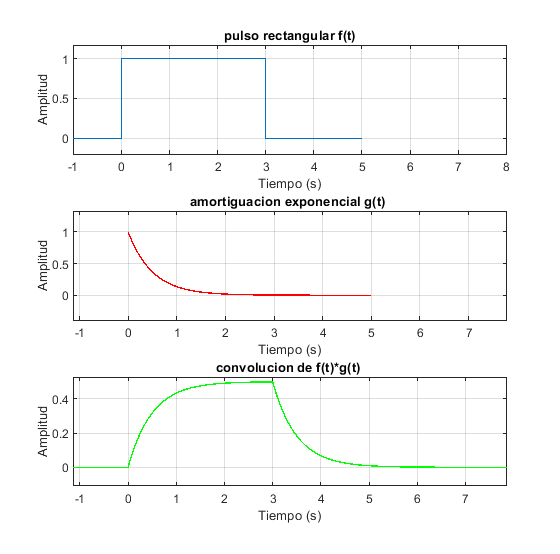
\includegraphics[scale=0.8]{fig9.png}
    \caption{convolucion de $f(t)*g(t)$ }
\end{figure}
\newpage










\empty{\underline{\textbf{$f(t)*h(t)$= $\int_{-\infty}^{\infty} h(\tau)f(t-\tau) d\tau  $}}}\newline


sabemos que :\newline \newline
$u_{n}(t)*u_{m}(t)=u_{n+m+1}(t)$\newline
$u_{n}(t-a)*u_{m}(t-b)=u_{n+m+1}(t-a-b)$\newline\newline
$f(t)=rectpuls(t-1.5)\ = u_0(t)-u_0(t-3)$\newline 
$h(t)=tripuls(t-1) \ = u_1(t)-2u_1(t-1)+u_1(t-2)$\newline 

$f(t)*h(t)=(u_0(t)-u_0(t-3))*(u_1(t)-2u_1(t-1)+u_1(t-2))$\newline
$f(t)*h(t) \ =u_2(t)-2u_2(t-1)+u_2(t-2)-u_2(t-3)+2u_2(t-4)-u_2(t-5)$\newline \newline
la grafica de $f(t)*h(t) es $

\begin{figure}[H]
    \centering
    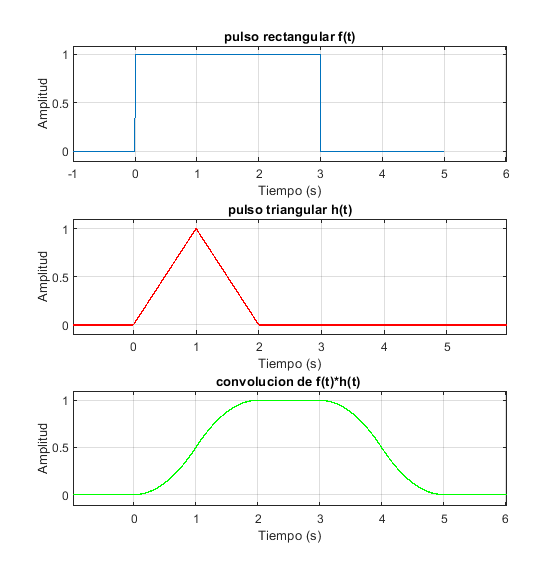
\includegraphics[scale=0.9]{fig10.png}
    \caption{convolucion de $f(t)*h(t)$ }
\end{figure}  \newpage
la grafica de $g(t)*h(t)$\newline \newline
\begin{figure}[H]
    \centering
    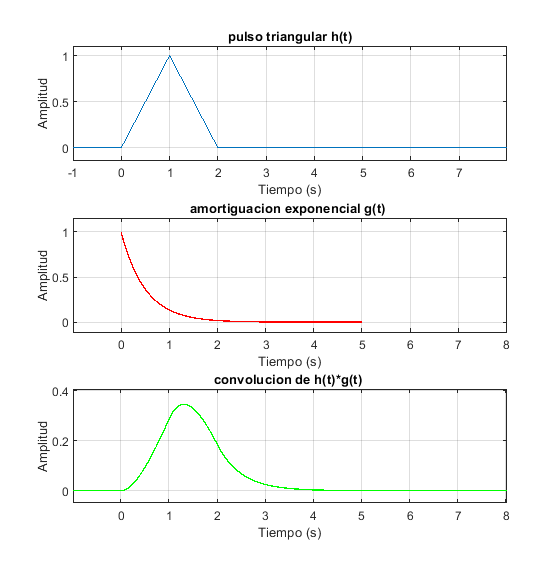
\includegraphics[scale=1.1]{fig11.png}
    \caption{convolucion de $f(t)*h(t)$ }
\end{figure}
\newpage










Ahora usando \textbf{matlab} y el comando \textit{conv}  hallaremos las convoluciones de $f(t)*f(t),\ f(t)*g(t), \ g(t)*g(t),\ g(t)*h(t),\ h(t)*h(t)$
\newline \newline
\textbf{$f(t)*f(t)$}
\begin{figure}[H]
    \centering
    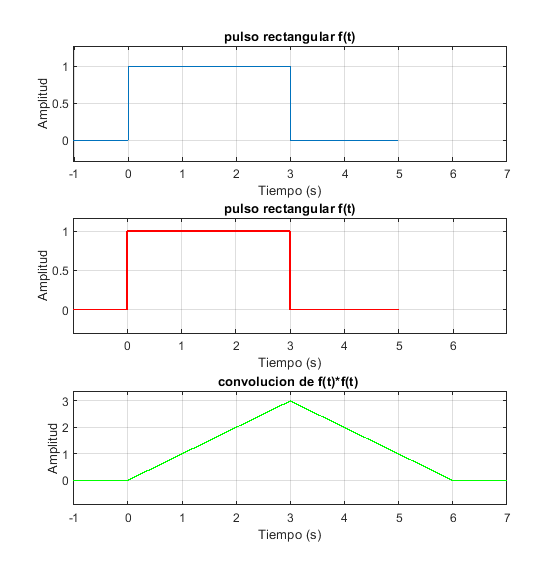
\includegraphics[scale=1.2]{fig12.png}
    \caption{convolucion de $h(t)*h(t)$ }
\end{figure}
\newpage
\textbf{$f(t)*g(t)$}
\begin{figure}[H]
    \centering
    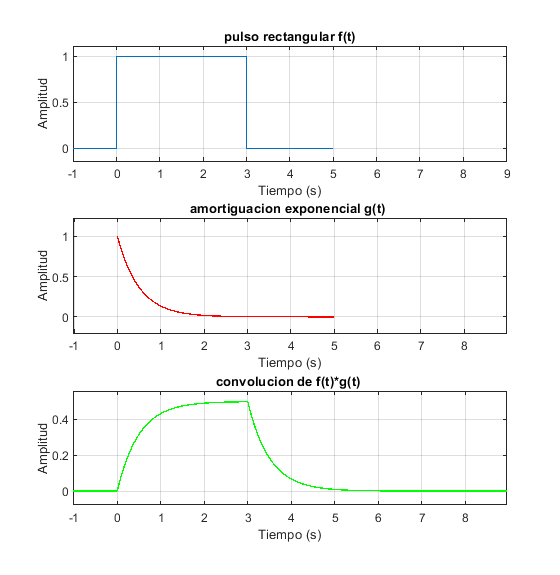
\includegraphics[scale=1.2]{fig13.png}
    \caption{convolucion de $f(t)*h(t)$ }
\end{figure}
\newpage
\textbf{$g(t)*g(t)$}
\begin{figure}[H]
    \centering
    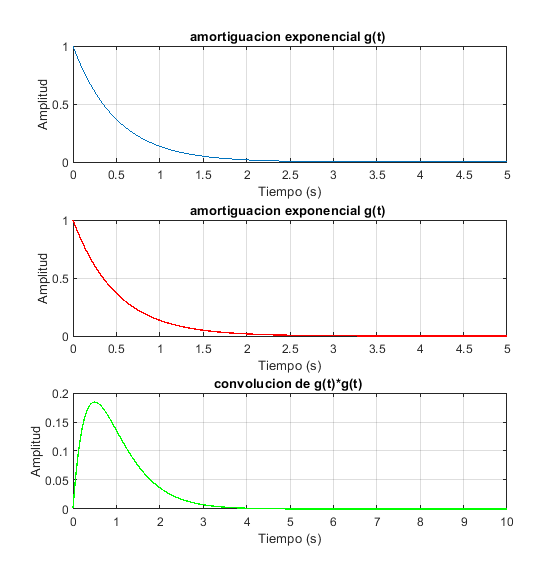
\includegraphics[scale=1.2]{fig14.png}
    \caption{convolucion de $g(t)*g(t)$ }
\end{figure} 
\newpage
\textbf{$g(t)*h(t)=h(t)*g(t)$}
\begin{figure}[H]
    \centering
    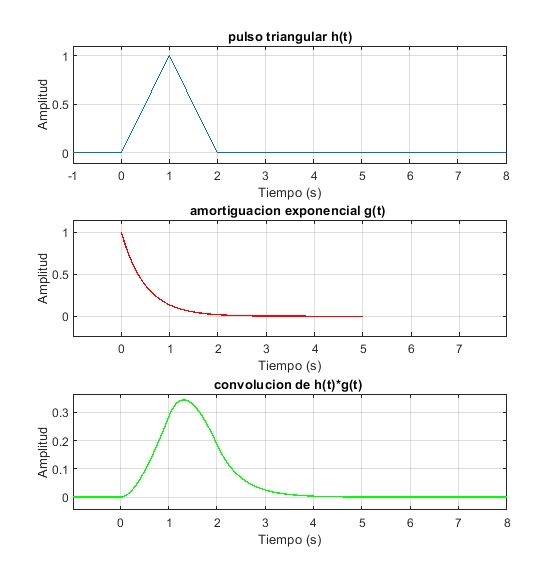
\includegraphics[scale=1.2]{fig15.png}
    \caption{convolucion de $g(t)*g(t)$ }
\end{figure} 
\newpage
\textbf{$h(t)*h(t)=h(t)*h(t)$}

\begin{figure}[H]
    \centering
    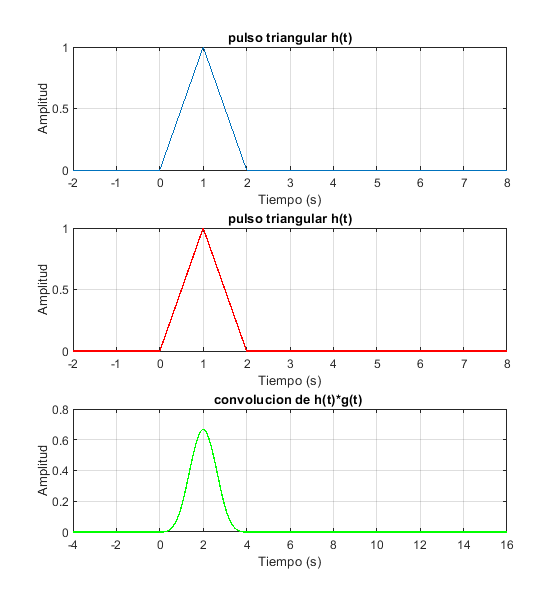
\includegraphics[scale=1.2]{fig16.png}
    \caption{convolucion de $h(t)*g(t)$ }
\end{figure}
	\newpage
	%Problema 2
	\item[\textbf{2.}]
	\textbf{Sea $f[n]=3$ , $0\leq n \leq 2$, un pulso cuadrado , $g[n]=[1,2,3,2,1]$ un pulso triangular , sea $h[n]=(\frac{1}{2})^n$ , $0\leq n\leq 8$ una amortiguación exponencial}
	\item[\textbf{a)}]
	\textbf{Usando el MATLAB grafique las señales en tiempo discreto f[n],g[n] y h[n].}\\
	$ \bullet$Para la gráfica $f[n]=3$ , $ 0\leq n\leq 2$, se utilizo la función stem de MATLAB para realizar un pulso cuadrado consideramos en un intervalo de $[-8,8]$.
\begin{figure}[h]
\centering
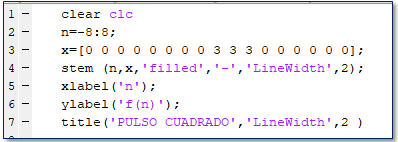
\includegraphics[scale=0.6]{../Imagenes de señales problema 2/Sin título.png} 
\end{figure}

\begin{figure}[h]
\centering
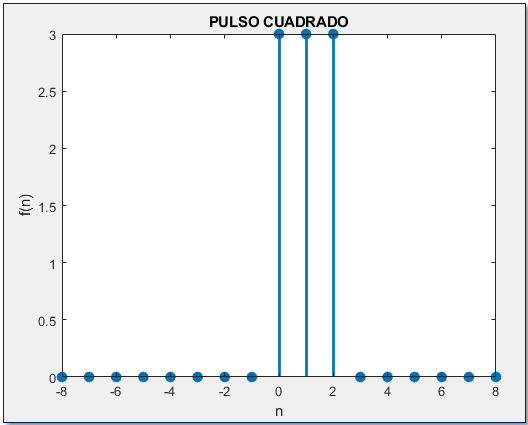
\includegraphics[scale=0.5]{../Imagenes de señales problema 2/pulso.png} 
\caption{Código en Matlab y gráfica de f[n]} 
\label{Gráfica_fn}
\end{figure}
$\bullet$Para la gráfica $g[n]=[1,2,3,2,1]$ , $-2\leq n\leq 2$, se utilizo la función stem de MATLAB para realizar un pulso rectangular consideramos en un intervalo de $[-8,8]$.

\begin{center}
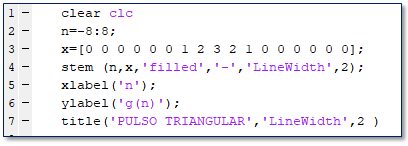
\includegraphics[scale=0.6]{../Imagenes de señales problema 2/sintutulo1.png}
\end{center}

\begin{figure}[h]
\centering
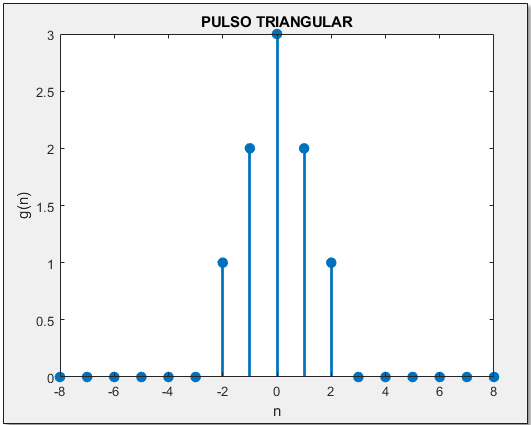
\includegraphics[scale=0.5]{../Imagenes de señales problema 2/triangulo.png} 
\caption{Código en Matlab y gráfica de g[n]} 
\label{Gráfica_gn}
\end{figure}
\newpage
$\bullet$Para la grafica $h[n]=(\frac{1}{2})^n$, se utilizo la funcion stem de MATLAB para realizar la amortiguación exponencial $[-8,8]$ con paso 1.
\begin{figure}[h]
\centering
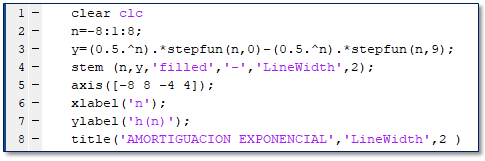
\includegraphics[scale=0.6]{../Imagenes de señales problema 2/titulo2.png} 
\label{Código_hn}
\end{figure}

\begin{figure}[h]
\centering
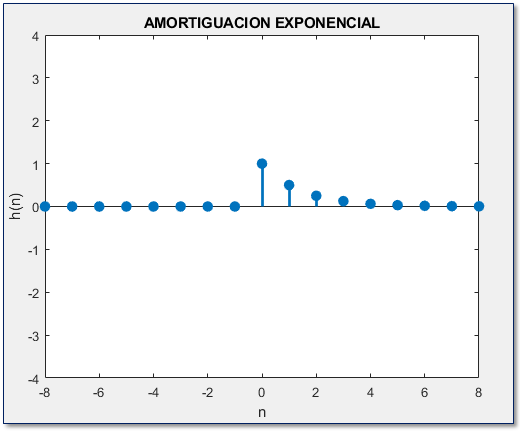
\includegraphics[scale=0.6]{../Imagenes de señales problema 2/expone.png} 
\caption{Código en Matlab y gráfica de h[n]}
\label{Gráfica_hn}
\end{figure}
	\item[\textbf{b)}]
	\textbf{Encuentre en términos de n y la señal escalón unitario las siguientes convoluciones:}\\
Como nos piden la convolución de dos señales discretas por conocimiento previo:
$$\boxed{y[n]=x[n]*h[n]=\sum_{k=-\infty}^{\infty}x[k]h[n-k]}$$
$\bullet$ Hallamos la convolución de $f[n]*g[n]$ con la formula previa hallada.
$$n<-2 \rightarrow y[n]=0$$
$$n=-2 \rightarrow y[n]=\sum_{k=-\infty}^{\infty}f[k]g[n-k]=f[0]g[-2]=(3)(1)=3$$
$$n=-1 \rightarrow y[n]=\sum_{k=-\infty}^{\infty}f[k]g[n-k]=f[0]g[-1]+f[1]g[-2]=9$$
$$n=0 \rightarrow y[n]=\sum_{k=-\infty}^{\infty}f[k]g[n-k]=f[0]g[n]+f[1]g[-1]+f[2]g[-2]=18$$
$$n=1 \rightarrow y[n]=\sum_{k=-\infty}^{\infty}f[k]g[n-k]=f[0]g[1]+f[1]g[0]+f[2]g[-1]=21$$
$$n=2 \rightarrow y[n]=\sum_{k=-\infty}^{\infty}f[k]g[n-k]=f[0]g[2]+f[1]g[1]+f[2]g[0]=18$$
$$n=3 \rightarrow y[n]=\sum_{k=-\infty}^{\infty}f[k]g[n-k]=f[1]g[2]+f[2]g[1]=9$$\\
$$n=4 \rightarrow y[n]=\sum_{k=-\infty}^{\infty}f[k]g[n-k]=f[2]g[2]=3$$\\
$$n>4 \rightarrow y[n]=0$$
\begin{equation*}
y[n]=f[n]*g[n] =
\begin{cases}
0 & \text{si $n<-2 $}\\
3 & \text{si $n= -2$}\\
9 & \text{si $n= -1$}\\
18 & \text{si $n= 0$}\\
21 & \text{si $n= 1$}\\
18 & \text{si $n= 2$}\\
9 & \text{si $n= 3$}\\
3 & \text{si $n=4$}\\
0 & \text{si $n>4$}
\end{cases}
\end{equation*}\\
\textbf{Expresamos en n y escalón unitario la señal:}
$$\boxed{y[n]=3u[n+2]+6u[n+1]+9u[n]+3u[n-1]-3u[n-2]-9u[n-3]-6u[n-4]-3u[n-5]}$$

$\bullet$ Hallamos la convolución de $f[n]*h[n]$ con la formula previa hallada.
$$f[n]*h[n]=\sum_{k=-\infty}^{\infty}f[k]h[n-k]$$
$$n<0 \rightarrow y[n]=0$$
$$n=0 \rightarrow y[n]=\sum_{k=-\infty}^{\infty}f[k]h[n-k]=f[0]h[0]=3$$
$$n=1 \rightarrow y[n]=\sum_{k=-\infty}^{\infty}f[k]h[n-k]=f[0]h[1]+f[1]h[0]=\frac{9}{2}$$
$$n=2 \rightarrow y[n]=\sum_{k=-\infty}^{\infty}f[k]h[n-k]=f[0]h[2]+f[1]h[1]+f[2]h[0]=\frac{21}{4}$$
$$n=3 \rightarrow y[n]=\sum_{k=-\infty}^{\infty}f[k]h[n-k]=f[0]h[3]+f[1]h[2]+f[2]h[1]=\frac{21}{8}$$
$$n=4 \rightarrow y[n]=\sum_{k=-\infty}^{\infty}f[k]h[n-k]=f[0]h[4]+f[1]h[3]+f[2]h[2]=\frac{21}{16}$$
$$n=5 \rightarrow y[n]=\sum_{k=-\infty}^{\infty}f[k]h[n-k]=f[0]h[5]+f[1]h[4]+f[2]h[3]=\frac{21}{32}$$
$$n=6 \rightarrow y[n]=\sum_{k=-\infty}^{\infty}f[k]h[n-k]=f[0]h[6]+f[1]h[5]+f[2]h[4]=\frac{21}{64}$$
$$n=7 \rightarrow y[n]=\sum_{k=-\infty}^{\infty}f[k]h[n-k]=f[0]h[7]+f[1]h[6]+f[2]h[5]=\frac{21}{128}$$
$$n=8 \rightarrow y[n]=\sum_{k=-\infty}^{\infty}f[k]h[n-k]=f[0]h[8]+f[1]h[7]+f[2]h[6]=\frac{21}{256}$$
$$n=9 \rightarrow y[n]=\sum_{k=-\infty}^{\infty}f[k]h[n-k]=f[1]h[8]+f[2]h[7]=\frac{9}{256}$$
$$n=10 \rightarrow y[n]=\sum_{k=-\infty}^{\infty}f[k]h[n-k]=f[2]h[8]=\frac{3}{256}$$
$$n>10 \rightarrow y[n]=\sum_{k=-\infty}^{\infty}f[k]h[n-k]=0$$
\begin{equation*}
y[n]=f[n]*h[n] =
\begin{cases}
0 & \text{si $n<0 $}\\
3 & \text{si $n= 0$}\\
\frac{9}{2} & \text{si $n= 1$}\\
\frac{21}{4} & \text{si $n= 2$}\\
\frac{21}{8} & \text{si $n= 3$}\\
\frac{21}{16} & \text{si $n= 4$}\\
\frac{21}{32} & \text{si $n= 5$}\\
\frac{21}{64} & \text{si $n=6$}\\
\frac{21}{128} & \text{si $n=7$}\\
\frac{21}{256} & \text{si $n=8$}\\
\frac{9}{256} & \text{si $n=9$}\\
\frac{3}{256} & \text{si $n=10$}\\
0 & \text{si $n>10$}
\end{cases}
\end{equation*}\\
\textbf{Expresamos en n y escalón unitario la señal:}
$$\boxed{y[n]=(0.5)^n(3u[n]+6u[n-1]+12u[n-2]-12u[n-9])-(0.5)^8(6u[n-10]-3u[n-11])}$$
$\bullet$ Hallamos la convolución de $g[n]*h[n]$ con la formula previa hallada.
$$g[n]*h[n]=\sum_{k=-\infty}^{\infty}g[k]h[n-k]$$
$$n<-2 \rightarrow y[n]=0 $$
$$n=-2 \rightarrow y[n]=\sum_{k=-\infty}^{\infty}g[k]h[n-k]=g[-2]h[0]=1 $$
$$n=-1 \rightarrow y[n]= \sum_{k=-\infty}^{\infty}g[k]h[n-k]=g[-1]h[0]+g[-2]h[1]=\frac{5}{2} $$
$$n=0 \rightarrow y[n]= \sum_{k=-\infty}^{\infty}g[k]h[n-k]=g[-2]h[2]+g[-1]h[1]+g[0]h[0]=\frac{17}{4} $$
$$n=1 \rightarrow y[n]= \sum_{k=-\infty}^{\infty}g[k]h[n-k]=g[-2]h[3]+g[-1]h[2]+g[0]h[1]+g[1]h[0]=\frac{33}{8} $$
$$n=2 \rightarrow y[n]= \sum_{k=-\infty}^{\infty}g[k]h[n-k]=g[-2]h[4]+g[-1]h[3]+g[0]h[2]+g[1]h[1]+g[2]h[0]=\frac{49}{16} $$
$$n=3 \rightarrow y[n]= \sum_{k=-\infty}^{\infty}g[k]h[n-k]=g[-2]h[5]+g[-1]h[4]+g[0]h[3]+g[1]h[2]+g[2]h[1] =\frac{49}{32}$$
$$n=4 \rightarrow y[n]= \sum_{k=-\infty}^{\infty}g[k]h[n-k]=g[-2]h[6]+g[-1]h[5]+g[0]h[4]+g[1]h[3]+g[2]h[2]=\frac{49}{64} $$
$$n=5 \rightarrow y[n]= \sum_{k=-\infty}^{\infty}g[k]h[n-k]=g[-2]h[7]+g[-1]h[6]+g[0]h[5]+g[1]h[4]+g[2]h[3]=\frac{49}{128} $$
$$n=6 \rightarrow y[n]= \sum_{k=-\infty}^{\infty}g[k]h[n-k]=g[-2]h[8]+g[-1]h[7]+g[0]h[6]+g[1]h[5]+g[2]h[4]=\frac{49}{256} $$
$$n=7 \rightarrow y[n]= \sum_{k=-\infty}^{\infty}g[k]h[n-k]=g[-1]h[8]+g[0]h[7]+g[1]h[6]+g[2]h[5]=\frac{3}{32} $$
$$n=8 \rightarrow y[n]= \sum_{k=-\infty}^{\infty}g[k]h[n-k]=g[0]h[8]+g[1]h[7]+g[2]h[6] =\frac{11}{256}$$
$$n=9 \rightarrow y[n]= \sum_{k=-\infty}^{\infty}g[k]h[n-k]=g[1]h[8]+g[2]h[7]=\frac{1}{64} $$
$$n=10 \rightarrow y[n]= \sum_{k=-\infty}^{\infty}g[k]h[n-k]=g[2]h[8]=\frac{1}{256}$$
$$n>10 \rightarrow y[n]=0 $$
\begin{equation*}
y[n]=g[n]*h[n] =
\begin{cases}
0 & \text{si $n<-2 $}\\
1 & \text{si $n= -2$}\\
\frac{5}{2} & \text{si $n= -1$}\\
\frac{17}{4} & \text{si $n= 0$}\\
\frac{33}{8} & \text{si $n= 1$}\\
\frac{49}{16} & \text{si $n= 2$}\\
\frac{49}{32} & \text{si $n= 3$}\\
\frac{49}{64} & \text{si $n=4$}\\
\frac{49}{128} & \text{si $n=5$}\\
\frac{49}{256} & \text{si $n=6$}\\
\frac{3}{32} & \text{si $n=7$}\\
\frac{11}{256} & \text{si $n=8$}\\
\frac{1}{64} & \text{si $n=9$}\\
\frac{1}{256} & \text{si $n=10$}\\
0 & \text{si $n>10$}
\end{cases}
\end{equation*}\\
\textbf{Expresamos en n y escalón unitario la señal:}
$$y[n]=(0.5)^n(u[n+2]+4u[n+1]+12u[n]+16u[n-1]+16u[n-2]-49u[n-7])$$ $$+(0.5)^5(3u[n-7]-3u[n-8])
+(0.5)^8(11u[n-8]-11u[n-9])$$ $$+(0.5)^6(u[n-9]-u[n-10])+(0.5)^8(u[n-10]-u[n-11])$$
	\item[\textbf{c)}]	
	\textbf{Usando el comando conv en MATLAB grafique las convoluciones $$f[n]*f[n],f[n]*g[n],f[n]*h[n],g[n]*g[n], g[n]*h[n],h[n]*h[n]$$}
\textbf{Graficando}\\
 Como el algoritmo es igual para todos, solo bosquejamos las gráficas: 
\begin{center}
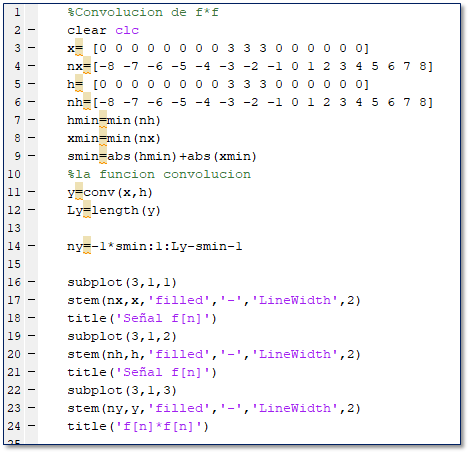
\includegraphics[scale=0.70]{../Imagenes de señales problema 2/ff.png} 
\end{center}
$$Convolucion :f[n]*f[n]$$ 
\begin{center}
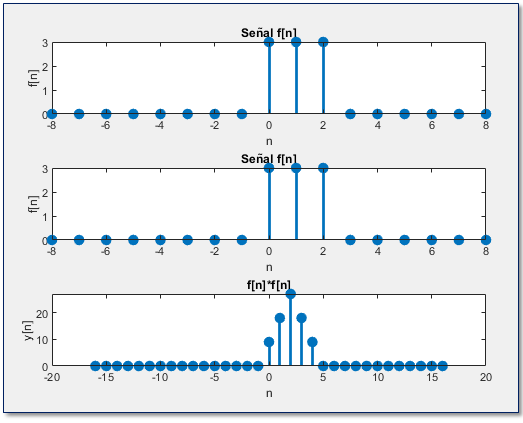
\includegraphics[scale=0.80]{../Imagenes de señales problema 2/ffgrafica.png} 
\end{center}
\newpage
$$Convolucion :f[n]*g[n]$$
\begin{center}
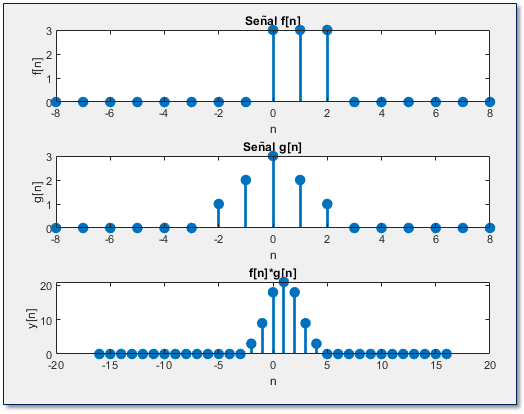
\includegraphics[scale=0.80]{../Imagenes de señales problema 2/fggrafica.png} 
\end{center}
$$Convolucion :f[n]*h[n]$$
\begin{center}
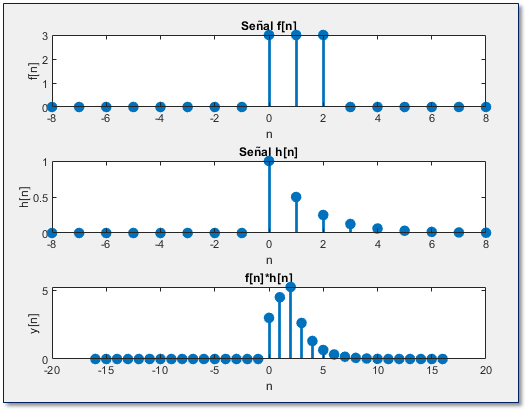
\includegraphics[scale=0.80]{../Imagenes de señales problema 2/fh.png} 
\end{center}
\newpage
$$Convolucion :g[n]*g[n]$$
\begin{center}
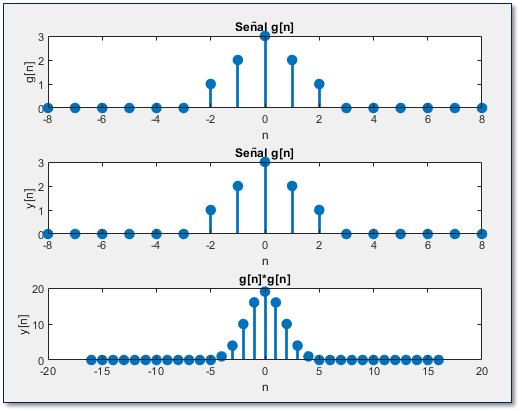
\includegraphics[scale=0.80]{../Imagenes de señales problema 2/gg.png} 
\end{center}
$$Convolucion :g[n]*h[n]$$
\begin{center}
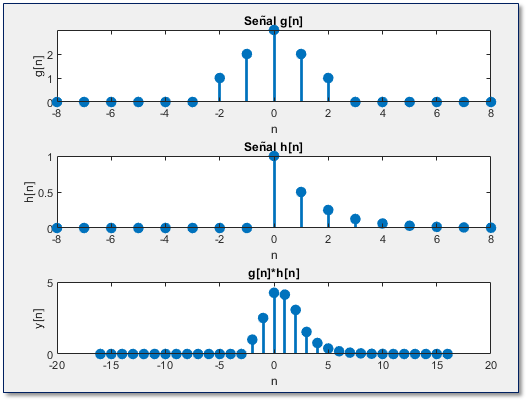
\includegraphics[scale=0.80]{../Imagenes de señales problema 2/gh.png} 
\end{center}
\newpage
$$Convolucion :h[n]*h[n]$$
\begin{center}
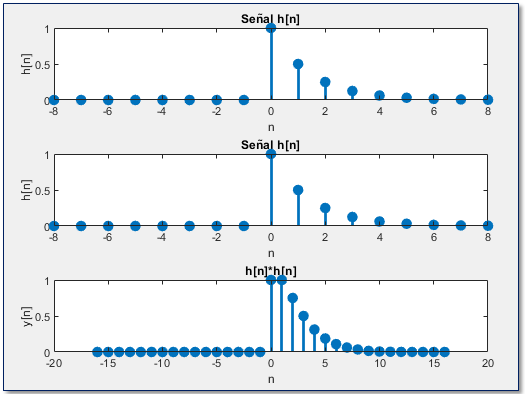
\includegraphics[scale=0.8]{../Imagenes de señales problema 2/hh.png} 
\end{center}
	\newpage
	
	%Pregunta 3
	\item[\textbf{3.}]\textbf{Considere un sistema causal LTI cuya entrada X[n] y salida Y[n] satisfacen $$6Y[n]-5Y[n-1]+Y[n-2]=6X[n]-4X[n-1]$$}
	\item[\textbf{a)}]
	\textbf{Usando la Transformada Z encuentre un diagrama de bloques para dichos sistema. Usando el Simulink y el diagrama de bloques encuentre la respuesta del sistema al impulso $X_{1}[n]=\delta[n]$ , al escalón unitario $X_{2}(t)=u[n]$ , y $X_{3}(t)=(\dfrac{1}{2})^2 u[n]$.}\\\\
    $\bullet$ \textbf{Realizando el diagrama de bloques del sistema causal LTI}\\\\
    \textbf{1er paso:} Aplicando la transformada Z 
    $$\mathcal{Z}\{6y[n]-5y[n-1]+y[n-2]=6x[n]-4x[n-1]\}$$   
    $$6Y(z)-5z^{-1}Y(z)+z^{-2}Y(z)=6X(z)-4z^{-1}X(z)$$  
    $$[6-5z^{-1}+z^{-2}]Y(z)=[6-4z^{-1}]X(z)$$   
    $$H(z)=\frac{Y(z)}{X(z)}=\frac{6-4z^{-1}}{6-5z^{-1}+z^{-2}}=\frac{2z(3z-2)}{6z^2-5z+1}=2z[\frac{3z-2}{(3z-1)(2z-1)}]=2z[\frac{3}{3z-1}-\frac{1}{2z-1}]$$
    \textbf{Función transferencia:}
    \begin{center}
    \boxed{H(z)=2(\frac{z}{z-1/3})-(\frac{z}{z-1/2})}
    \end{center}
    Donde se sabe que la entrada de $x_m[n]$ se relaciona con la salida $y_m[n]$ por medio de:  
    $$x_m[n]*h[n]=y_m[n]$$
    o con la transformada Z
    $$X_m(z)H(z)=Y_m(z)$$

	\textbf{2do paso: } Realizando el diagrama de bloques
	\begin{figure}[h]
	\centering
	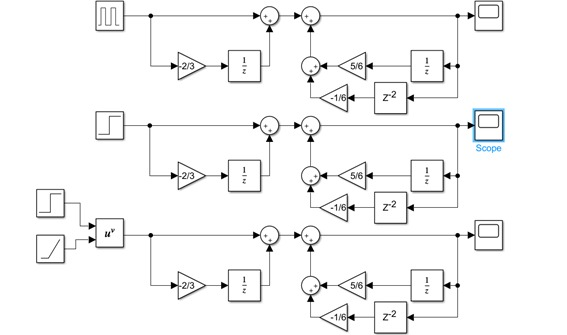
\includegraphics[scale=0.7]
{ DIAGRAMADEBLOQUESSISTEMA3} 
	\caption{Diagrama de bloque del sistema causal LTI, con las entradas pedidas}
\label{ DIAGRAMADEBLOQUESSISTEMA3}
\end{figure}
	\newpage
	%Respuestas y graficos

	$\bullet$\textbf{Respuesta al impulso($x_1(t)= \delta[n]$)}\\\\
	Si $x_1[n]=\delta[n]$ entonces $X_1(z)=1$; por lo que, $Y_1(z)=H(z)=2(\frac{z}{z-1/3})-(\frac{z}{z-1/2})$
	
	\begin{figure}[h]
	\centering
	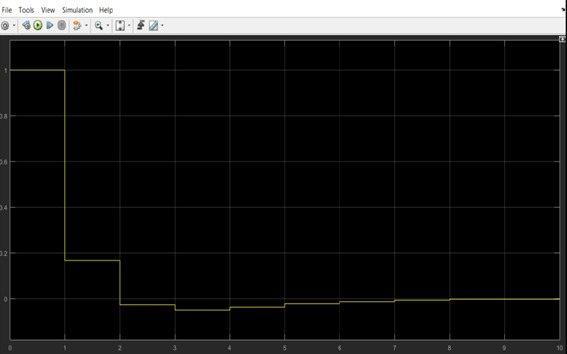
\includegraphics[scale=0.6]
{IMAGENRESPUESTAIMPULSO} 
	\caption{Gráfica de la respuesta al impulso}
\label{IMAGENRESPUESTAIMPULSO}
\end{figure}

	$\bullet$\textbf{Respuesta al escalón($x_2(n)= u[n]$)}\\\\
	 si $x_2[n]=u[n]$ entonces $X_2(z)=\frac{z}{z-1}$; por lo que, $Y_2(z)=\frac{z}{z-1}H(z)=2z[\frac{3z^2-2z}{(z-1)(3z-1)(2z-1)}]$        
     $$Y_2(z)=z[\frac{2}{2z-1}-\frac{3}{3z-1}+\frac{1}{z-1}]=\frac{z}{z-1/2}-\frac{z}{z-1/3}+\frac{z}{z-1}]$$

	\begin{figure}[h]
	\centering
	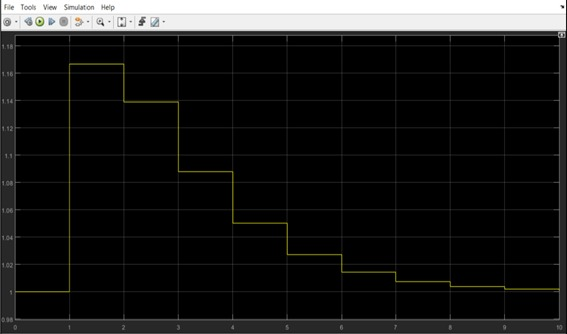
\includegraphics[scale=0.6]
{IMAGENRESPUESTAESCALON} 
	\caption{Gráfica de la respuesta al escalón}
\label{IMAGENRESPUESTAESCALON}
\end{figure}
	\newpage
	
	$\bullet$\textbf{Respuesta a $x_3[n]=(\frac{1}{2})^nu[n]$}\\\\
	si $x_3[n]=(\frac{1}{2})^nu[n]$ entonces $X_3(z)=\frac{2z}{2z-1}$; por lo que, $Y_3=\frac{2z}{2z-1}H(z)=4z[\frac{3z^2-2z}{(3z-1)(2z-1)^2}]$
        $$Y_3(z)=z[-\frac{12}{3z-1}+\frac{10}{2z-1}-\frac{2}{(2z-1)^2}]=-4\frac{z}{z-1/3}+5\frac{z}{z-1/2}-\frac{1}{2}\frac{z}{(z-1/2)^2}$$

	\begin{figure}[h]
	\centering
	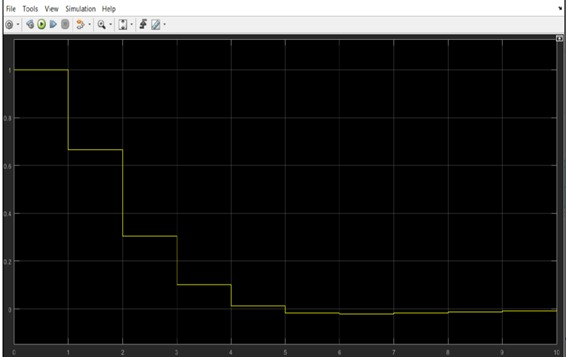
\includegraphics[scale=0.55]
{IMAGENRESPUESTAUEX} 
	\caption{Gráfica de la respuesta a $x_3[n]=(\frac{1}{2})^nu[n]$}
\label{IMAGENRESPUESTAUEX}
\end{figure}
	
	\item[\textbf{b)}]
	 \textbf{Encuentre las respuestas de la parte (a) en función de n.}\\
	  \textbf{1er paso:} Aplicando la transformada inversa de Z
	  
        $\bullet$\textbf{Respuesta al impulso($x_1(t)= \delta[n]$)}\\
        $$\mathcal{Z}^{-1}\{Y_1(z)=2(\frac{z}{z-1/3})-(\frac{z}{z-1/2})\}$$
   Entonces obtenemos la siguiente respuesta:
         \begin{center}
	$\therefore$ \boxed{y_1[n]=[2(\frac{1}{3})^n-(\frac{1}{2})^n]u[n]}
	\end{center}
            
	$\bullet$\textbf{Respuesta al escalón($x_2(n)= u[n]$)}\\
        $$\mathcal{Z}^{-1}\{Y_2(z)=\frac{z}{z-1/2}-\frac{z}{z-1/3}+\frac{z}{z-1}\}$$
        Entonces obtenemos la siguiente respuesta:
         \begin{center}
	$\therefore$ \boxed{y_2[n]=[(\frac{1}{2})^n-(\frac{1}{3})^n+1]u[n]}
	\end{center} 
        
        $\bullet$\textbf{Respuesta a $x_3[n]$}\\
        $$\mathcal{Z}^{-1}\{Y_3(z)=-4\frac{z}{z-1/3}+5\frac{z}{z-1/2}-\frac{1}{2}\frac{z}{(z-1/2)^2}\}$$
         
     Entonces obtenemos la siguiente respuesta:
	\begin{center}
	$\therefore$ \boxed{y_3[n]=[-4(\frac{1}{3})^n+5(\frac{1}{2})^n-(\frac{1}{2})^nn]u[n]}
	\end{center} 

	\newpage
	
	%Pregunta 4
	\item[\textbf{4.}]\textbf{Considere un sistema causal LTI cuya entrada X(t) y salida Y(t) satisfacen $$Y^{''}(t)+2Y^{'}(t)+Y(t)=2X^{'}(t)+X(t)$$}
	
	\item[\textbf{a)}]
	\textbf{Usando la Transformada de Laplace encuentre un diagrama de bloques para dichos sistema. Usando el Simulink y el diagrama de bloques encuentre la respuesta del sistema al impulso $X_{1}(t)=\delta(t)$ , al escalón unitario $X_{2}(t)=u(t)$ , y a la amortiguación $X_{3}(t)=exp(-2t)$.}\\\\
	\textbf{$\bullet$ Realizando el diagrama de bloques del sistema causal LTI }\\\\
	\textbf{1er paso:} Calculando la función de transferencia del sistema.
	$$Y^{''}(t)+2Y^{'}(t)+Y(t)=2X^{'}(t)+X(t)$$
Aplicando la transformada de Laplace
%Simbolo para la transformada  de Laplace(\mathcal{L})
	\begin{eqnarray}
	\label{TransLaplaceDelSistema}
		\mathcal{L}{\lbrace Y^{''}(t)\rbrace}+2 \mathcal{L}{ \lbrace Y^{'}(t)\rbrace}+ \mathcal{L}{ \lbrace Y(t)\rbrace }=2 \mathcal{L}{\lbrace X^{'}(t)\rbrace}+ \mathcal{L}{ \lbrace X(t) \rbrace}
	\end{eqnarray}
	\textbf{Importante:} Transformada de Laplace que aplicaremos en (\ref{TransLaplaceDelSistema})\\ 
	$$\mathcal{L}{\lbrace Y^{''}(t)\rbrace}=s^2f(s)-sF(0)-F^{'}(0)$$
	$$\mathcal{L}{ \lbrace Y^{'}(t)\rbrace}=sf(s)-F(0)$$
	Para este sistema causal LTI, consideraremos que $F(0)=0$ y $F^{'}(0)=0$; por lo tanto, obtendremos lo siguiente:
	\begin{eqnarray}
	\label{TransLaplaceDe2Derivada}
		\mathcal{L}{\lbrace Y^{''}(t)\rbrace}=s^2f(s)
	\end{eqnarray}
	\begin{eqnarray}
	\label{TransLaplaceDe1Derivada}
		\mathcal{L}{ \lbrace Y^{'}(t)\rbrace}=sf(s)
	\end{eqnarray}
	Aplicando la transfomadas de Laplace (\ref{TransLaplaceDe1Derivada})
y (\ref{TransLaplaceDe2Derivada}) en la EDO (\ref{TransLaplaceDelSistema})
	$$s^2y(s)+2sy(s)+y(s)=2sx(s)+x(s)$$
	$$y(s)+ \dfrac{2y(s)}{s}+ \dfrac{y(s)}{s^2}= \dfrac{2x(s)}{s}+ \dfrac{x(s)}{s^2}$$
	\begin{eqnarray}
	\label{SistemaParaDBloque}
		y(s)= \dfrac{2x(s)}{s}+ \dfrac{x(s)}{s^2}- \dfrac{2y(s)}{s}- \dfrac{y(s)}{s^2}
	\end{eqnarray}
	\begin{eqnarray}
	\label{Función transferencia4}
	\boxed{h(s)=\dfrac{y(s)}{x(s)}=\dfrac{2s+1}{s^2 +2s+1}}
	\end{eqnarray}
	\newpage
\textbf{2do paso:}\\
Realizando el diagrama de bloques del sistema en Simulink, a partir de la ecuación (\ref{SistemaParaDBloque})
	
	\begin{figure}[h]
	\centering
	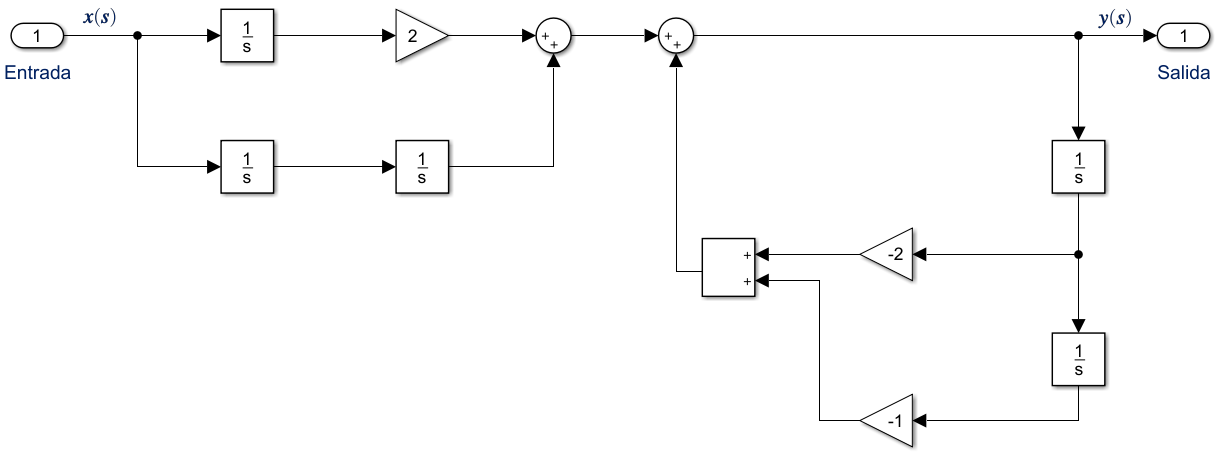
\includegraphics[scale=0.49]
{DIAGRAMABLOQUESISTEMA4} 
	\caption{Diagrama de bloque del sistema causal LTI}
\label{DIAGRAMABLOQUESISTEMA4}
\end{figure}
	
	Verificando si nuestro diagrama de bloque es correcta.
	\begin{figure}[h]
	\centering
	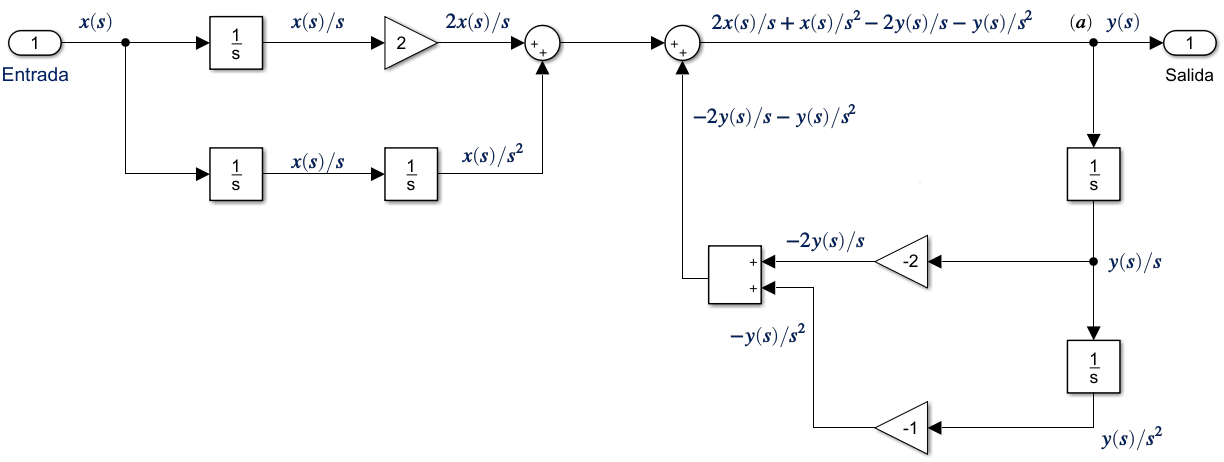
\includegraphics[scale=0.49]
{DIAGRAMABLOQUESISTEMA4VERIFICACION} 
	\caption{Verificacióndel diagrama de bloque del sistema causal LTI}
\label{DIAGRAMABLOQUESISTEMA4VERIFICACION}
\end{figure}\\
	Del diagrama de bloques de la figura (\ref{DIAGRAMABLOQUESISTEMA4VERIFICACION})
en (a), se verifica la ecuación (\ref{SistemaParaDBloque})\\
	$$y(s)= \dfrac{2x(s)}{s}+ \dfrac{x(s)}{s^2}- \dfrac{2y(s)}{s}- \dfrac{y(s)}{s^2}$$
	\newpage
 	$\bullet$ \textbf{Respuesta al impulso($X_1(t)=\delta (t))$}\\
	
	\begin{figure}[h]
	\centering
	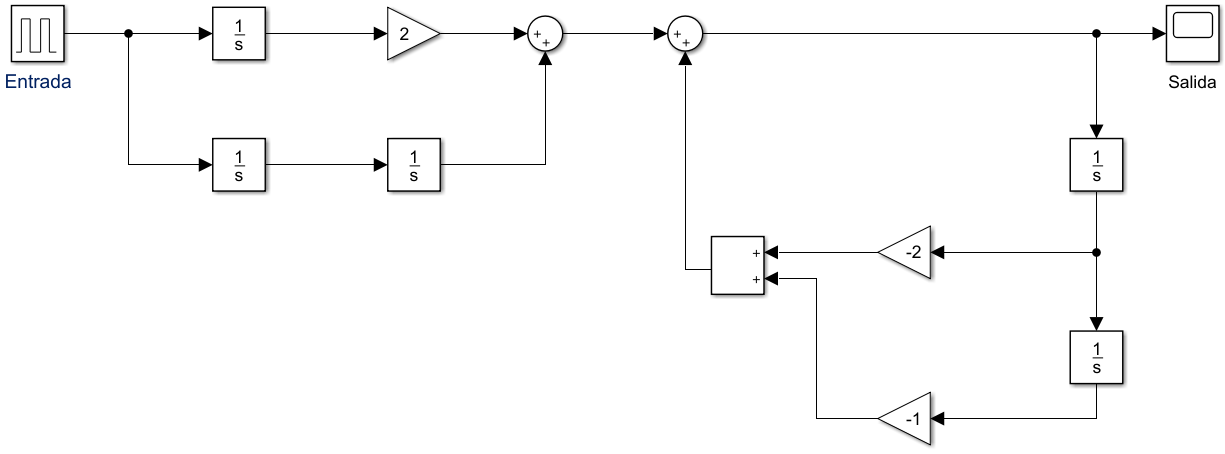
\includegraphics[scale=0.49]
{DIAGRAMADEIMPULSO} 
	\caption{Diagrama de bloques con entrada de un impulso}
\label{DIAGRAMADEIMPULSO}
\end{figure}
\begin{figure}[h]
	\centering
	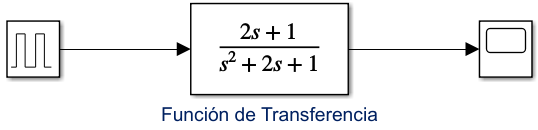
\includegraphics[scale=0.6]
{DIAGRAMADEIMPULSO2} 
	\caption{Otro diagrama de bloques con entrada de un impulso}
\label{DIAGRAMADEIMPULSO2}
\end{figure}
	Se puede verificar que en ambos diagramas de bloques se obtiene como respuesta, la siguiente señal con respecto al tiempo.
	\begin{figure}[h]
	\centering
	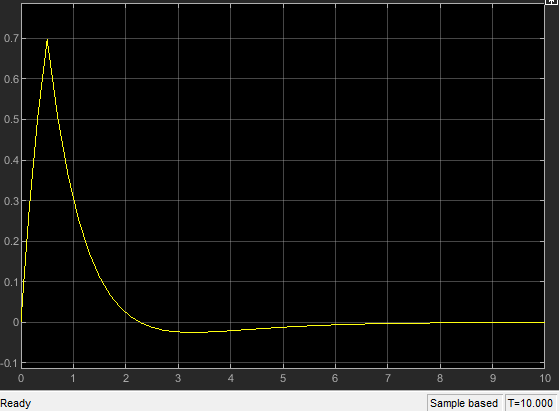
\includegraphics[scale=0.7]
{RESPUESTADELIMPULSO} 
	\caption{Gráfica de la respuesta al impulso}
\label{RESPUESTADELIMPULSO}
\end{figure}
	\newpage
	
	$\bullet$ \textbf{Respuesta al escalón($X_2(t)= u(t))$}\\
	
	\begin{figure}[h]
	\centering
	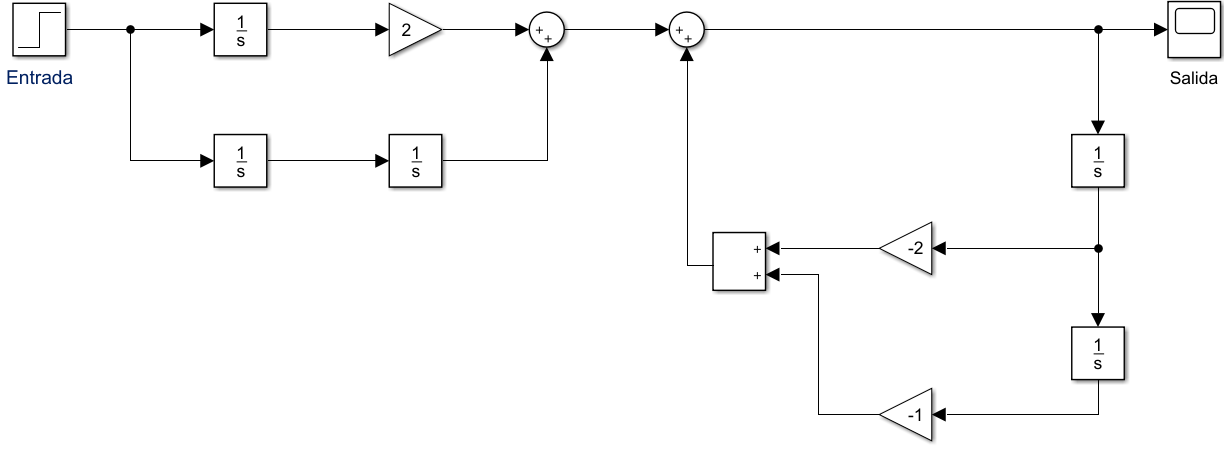
\includegraphics[scale=0.49]
{DIAGRAMADEESCALON} 
	\caption{Diagrama de bloques con entrada de un escalón}
\label{DIAGRAMADEESCALON}
\end{figure}
\begin{figure}[h]
	\centering
	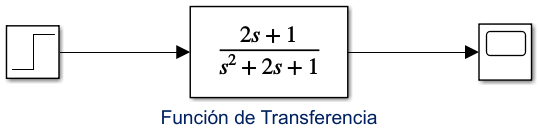
\includegraphics[scale=0.6]
{DIAGRAMADEESCALON2} 
	\caption{Otro diagrama de bloques con entrada de un escalón}
\label{DIAGRAMADEESCALON2}
\end{figure}
	Se puede verificar que en ambos diagramas de bloques se obtiene como respuesta, la siguiente señal con respecto al tiempo.
	\begin{figure}[h]
	\centering
	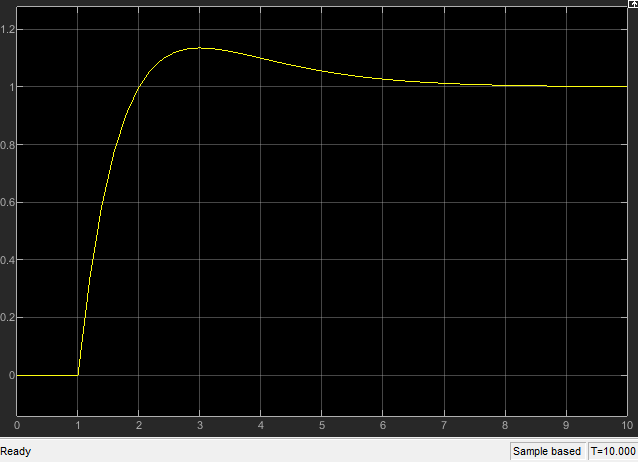
\includegraphics[scale=0.6]
{RESPUESTADELESCALON} 
	\caption{Gráfica de la respuesta al escalón}
\label{RESPUESTADELESCALON}
\end{figure}
	\newpage
	
	$\bullet$ \textbf{Respuesta a la amortiguación($X_3(t)= e^{-2t})$}\\
	
	\begin{figure}[h]
	\centering
	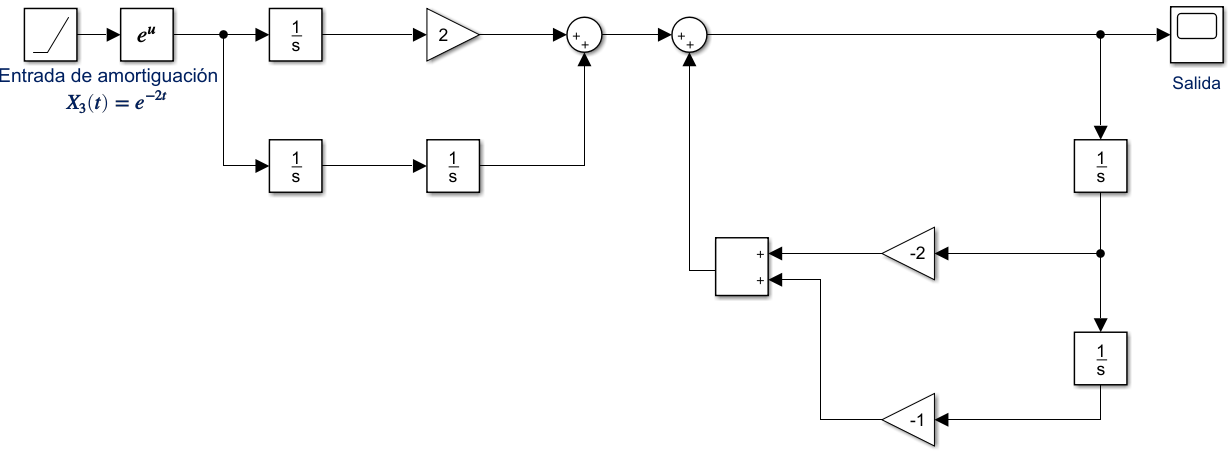
\includegraphics[scale=0.49]
{DIAGRAMADEAMORTIGUACION} 
	\caption{Diagrama de bloques con entrada de una amortiguación}
\label{DIAGRAMADEAMORTIGUACION}
\end{figure}
\begin{figure}[h]
	\centering
	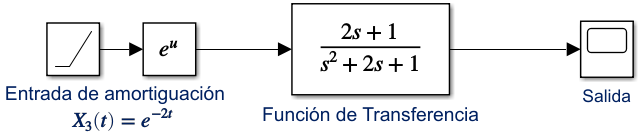
\includegraphics[scale=0.6]
{DIAGRAMADEAMORTIGUACION2} 
	\caption{Otro diagrama de bloques con entrada de una amortiguación}
\label{DIAGRAMADEAMORTIGUACION2}
\end{figure}
	Se puede verificar que en ambos diagramas de bloques se obtiene como respuesta, la siguiente señal con respecto al tiempo.
	\begin{figure}[h]
	\centering
	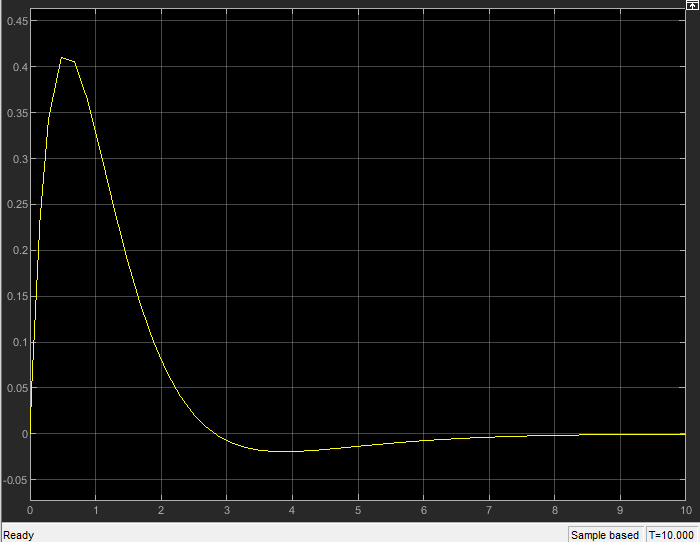
\includegraphics[scale=0.52]
{RESPUESTADEAMORTIGUACION} 
	\caption{Gráfica de la respuesta a la amortiguación}
\label{RESPUESTADEAMORTIGUACION}
\end{figure}
	\newpage
	\textbf{Importante:}\\\\
	Como en el programa de Simulink no se encuentra específicamente una entrada de amortiguación $X_3(t)= e^{-2t})$. Entonces, nosotros debemos realizar los siguientes pasos:\\
	\textbf{1er paso:} 
	Arrastrar al menú principal de Simulink los bloques de $e^u$ y la función rampa, que se encuentran en la librería de Simulink. Visualizar las siguientes imágenes:
	
	\begin{figure}[h]
	\centering
	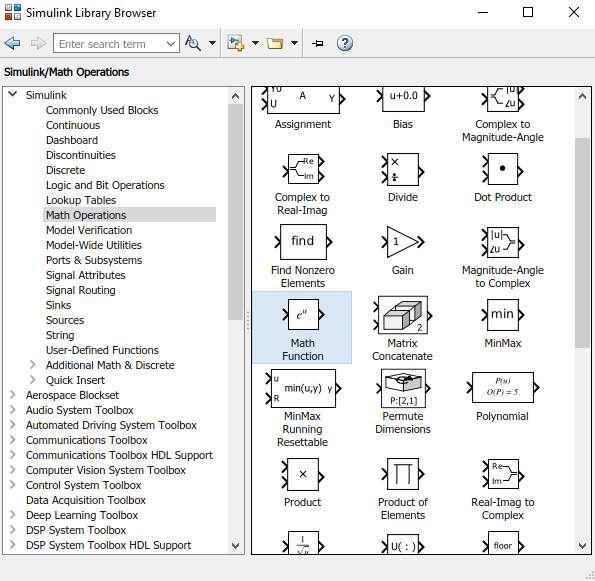
\includegraphics[scale=0.48]
{LOCALIZACIONDEEU} 
	\caption{Localización de $e^u$ en la librería de Simulink}
\label{LOCALIZACIONDEEU}
\end{figure}

	\begin{figure}[h]
	\centering
	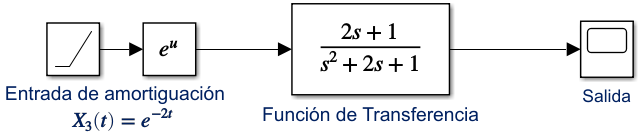
\includegraphics[scale=0.5]
{DIAGRAMADEAMORTIGUACION2} 
	\caption{Como debe quedar el diagrma de bloque del sistema}
\label{DIAGRAMADEAMORTIGUACION2}
\end{figure}
	\textbf{2do paso:} Configurar nuestra función rampa, para obtener $e^{-2t}$ como entrada. Donde el u de $e^u$ sera la función -2t.Luego debemos darle click a la función rampa, se nos abrirá una ventana (Visualizar (\ref{REALIZARLAAMORTIGUACIONENTRADA}))en el cual ingresaremos la pendiente de la recta -2t en la opción "Slope".
	
	\begin{figure}[h]
	\centering
	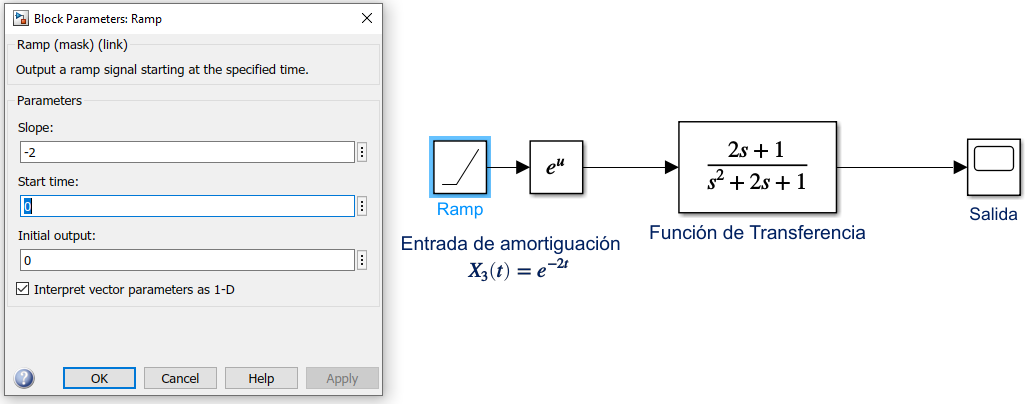
\includegraphics[scale=0.5]
{REALIZARLAAMORTIGUACIONENTRADA} 
	\caption{Configuración de nuestra función rampa}
\label{REALIZARLAAMORTIGUACIONENTRADA}
\end{figure}
	\textbf{Finalmente:} Ya estará lista nuestra entrada de amortiguación $X_3(t)= e^{-2t}$. 
	\newpage
	
	\item[\textbf{b)}]
	\textbf{Encuentre las respuestas de la parte (a)en términos de t}\\\\
	$\bullet$\textbf{Respuesta al impulso($X_1(t)=\delta (t))$}\\
	$$x_1(s)=\mathcal{L^{-}}{\lbrace \delta (t) \rbrace}=1$$
	A partir de la función de transferencia(\ref{Función transferencia4})aplicaremos lo anterior.
	$$\dfrac{y_1(s)}{x_1(s)}=\dfrac{2s+1}{s^2 +2s+1}$$
	$$\dfrac{y_1(s)}{1}=\dfrac{2}{s+1}-\dfrac{1}{(s+1)^2}$$
	Aplicando transformada inversa de Laplace
	$$\mathcal{L^{-}}{\lbrace y_1(s)\rbrace }=2 \mathcal{L^{-}}{\lbrace \dfrac{1}{s+1} \rbrace } -\mathcal{L^{-}}{\lbrace \dfrac{1}{(s+1)^2}\rbrace}$$
	$$Y_1(t)=2e^{-t}-te^{-t}$$
	Para $t \geq 0$, el $u(t)=1$, y para  $t < 0$, el $u(t)=0$\\
	Como el tiempo (t) es  mayor igual a 0. Entonces, obtendremos la siguiente respuesta del sistema\\\\
	\textbf{Respuesta al impulso:}
	\begin{center}
	$\therefore$ \boxed{Y_1(t)=(2e^{-t}-te^{-t})u(t)}
	\end{center}
	
	$\bullet$\textbf{Respuesta al escalón($X_2(t)= u(t))$}\\
	$$x_2(s)=\mathcal{L^{-}}{\lbrace u(t) \rbrace}= \dfrac{1}{s}$$
	A partir de la función de transferencia (\ref{Función transferencia4}) aplicaremos lo anterior.
	$$\dfrac{y_2(s)}{x_2(s)}= \dfrac{2s+1}{(s^2 +2s+1)} \rightarrow  y_2(s)= \dfrac{2s+1}{(s^2 +2s+1)(s)}$$
	$$ y_2(s)= \dfrac{1}{s}+ \dfrac{1}{(s+1)^2}- \dfrac{1}{s+1}$$
	Aplicando transformada inversa de Laplace
	$$\mathcal{L^{-}}{\lbrace y_2(s)\rbrace }= \mathcal{L^{-}}{\lbrace \dfrac{1}{s} \rbrace } +\mathcal{L^{-}}{\lbrace \dfrac{1}{(s+1)^2}\rbrace}-\mathcal{L^{-}}{\lbrace \dfrac{1}{s+1} \rbrace } $$
	$$Y_2(t)=1-te^{-t}-e^{-t}$$
	Para $t \geq 0$, el $u(t)=1$, y para  $t < 0$, el $u(t)=0$\\
	Como el tiempo (t) es  mayor igual a 0. Entonces, obtendremos la siguiente respuesta del sistema\\\\
	\textbf{Respuesta al escalón:}
	\begin{center}
	$\therefore$ \boxed{Y_2(t)=(1-te^{-t}-e^{-t})u(t)}
	\end{center}
	
	$\bullet$\textbf{Respuesta a la amortiguación($X_3(t)= e^{-2t})$}\\
	$$y_3(s)=\mathcal{L^{-}}{\lbrace e^{-2t} \rbrace}= \dfrac{1}{s+2}$$
	A partir de la función de transferencia(\ref{Función transferencia4})aplicaremos lo anterior.
	$$\dfrac{y_3(s)}{x_3(s)}= \dfrac{2s+1}{(s^2 +2s+1)} \rightarrow  y_2(s)= \dfrac{2s+1}{(s^2 +2s+1)(s+2)}$$
	$$ y_3(s)= - \dfrac{1}{(s+1)^2}+ \dfrac{3}{s+1} - \dfrac{3}{s+2}$$
	Aplicando transformada inversa de Laplace
	$$\mathcal{L^{-}}{\lbrace y_3(s)\rbrace }= - \mathcal{L^{-}}{\lbrace \dfrac{1}{(s+1)^2}\rbrace}+\mathcal{L^{-}}{\lbrace \dfrac{3}{s+1} \rbrace }-\mathcal{L^{-}}{\lbrace \dfrac{3}{s+2} \rbrace } $$
	$$Y_3(t)=-te^{-t}+3e^{-t}-3e^{-2t}$$
	Para $t \geq 0$, el $u(t)=1$, y para  $t < 0$, el $u(t)=0$\\
	Como el tiempo (t) es  mayor igual a 0. Entonces, obtendremos la siguiente respuesta del sistema\\\\
	\textbf{Respuesta a la amortiguación:}
	\begin{center}
	$\therefore$ \boxed{Y_3(t)=(-te^{-t}+3e^{-t}-3e^{-2t})u(t)}
	\end{center}
	\end{enumerate}
	}}
	
	\newpage
	\section{CONCLUSIONES}{
	\large{
	\begin{enumerate}
	\item[\textbf{b.}]
	\textbf{PREGUNTA 2}\\\\
	$\bullet$ Finalmente logre verificar los conceptos previos vistos en clases mediante el Software MATLAB .Como sabemos es un programa matemático que nos facilito los cálculos numéricos y gráficas. Fue de gran ayuda para comprobar y darnos una idea de la gráfica que se pueden generar entre la convoluci\'on de dos señales discretas vistos en la pregunta dos.\\
	
	\item[\textbf{c.}]
	\textbf{PREGUNTA 3}\\\\
	$\bullet$ La transformada inversa de la función de transferencia del sistema es la respuesta al impulso del sistema.\\
$\bullet$ Si en la respuesta del sistema el índice de la exponencial negativa (o suma de exponenciales negativas) es menor que la positiva (o suma de positiva), entonces la gráfica se va a ir por debajo del valor final para luego volver al valor final y ser cuasi constante.\\
$\bullet$ El valor final no necesariamente se va hacia el 0, si no depende de las condiciones iniciales, en específico sólo se reducen al 0 los que representan potencias menores que uno.\\


	\item[\textbf{d.}]
	\textbf{PREGUNTA 4}\\\\
	$\bullet$ El tiempo siempre es positivo; por ello, colocamos u(t) a nuestras respuestas ante una señal(impulso,escalón,amortiguador,...)
,ya que la función escalón se define de la siguiente manera.
	$$t \geq 0 \rightarrow u(t)=1$$
	$$t < 0 \rightarrow u(t)=0$$
	$\bullet$ La función de transferencia debido a la transformada de Laplace, es importante, ya que me permite graficar la respuesta ante una entrada (impulso,escalón,...), donde la gráfica será de la señal de salida respecto al tiempo. Cabe resaltar, que al realizar el diagrama de bloques en el programa de Simulink y darle una entrada, podremos visualizar nuestra gráfica de salida por medio de un "Scope" o un "osciloscopio".Debemos tener presente que la función de transferencia que proviene de una transformada z , Laplace y entre otras, es importante, ya que nos permite visualizar como nuestra señal de salida varia en el tiempo.
	\end{enumerate}
	}}
	\newpage
	\section{{BIBLIOGRAFIA}}{
	\large{
	\begin{enumerate}
	\item[\textbf{$\bullet$}]
	Antonio Artés Rodríguez,Fernando Pérez González. (2012). Comunicaciones digitales. 
	\item[\textbf{$\bullet$}]
López, H. I. (2009). Método Alternativo para Calcular la Convolución de Señales en Tiempo Continuo. 
\item[\textbf{$\bullet$}]
Oviedo, U. d. (2006). Simulación de sistemas de control continuos con MATLAB Y SIMULINK. 
\item[\textbf{$\bullet$}]
Miranda, J. (1983). MANUAL DE CALCULO diferencial é integral. 
	\end{enumerate}
	}}
\end{document}
	








